%
%	LaTeX - SCHABLONE fuer die SCHRIFTLICHE SEMINARAUSARBEITUNG
%		�EGST v3.14 � 12.09.2oo8
%
%%%	\documentclass[12pt]{article}
\documentclass[12pt,a4paper]{scrartcl}		% KOMA-Klassen benutzen!

\usepackage[ngerman]{babel}			% deutsche Namen/Umlaute
\usepackage[latin1]{inputenc}			% Zeichensatzkodierung
\usepackage{graphicx}				% Einbinden von Bildern
\usepackage{color}				% Farben wenn es sein mu�
\usepackage{amsmath}				% Mathematischer Formelsatz AMS
\usepackage{amsfonts}

%
%	HIER WERDEN TITEL REFERENT UND DATUM EINGETRAGEN
%
\newcommand\svthema{Kaltbl�ter in gro�st�dtischer Heimtierhaltung}
\newcommand\svperson{Steven Spielberg}
\newcommand\svdatum{14.~November 2008}
\newcommand\lvtyp{Proseminar im Wintersemester 2008}
\newcommand\lvname{Algorithmen der Mustererkennung und K�nstlichen Intelligenz}
\newcommand\lvinst{Institut f�r Informatik � FSU Jena}

\begin{document}

\title{ \textbf{\color{blue}\svthema} }
\author{ \textsl{\color{red}\svperson} --- \svdatum }
\date{ \small \textsc{"`\lvname"'} \\ {\lvtyp} � {\lvinst} }
\maketitle

%
%	AB HIER WIRD DER AUSARBEITUNGSTEXT EINGEFUEGT
%
\abstract{
	Hier steht eine kurze Zusammenfassung von circa 5--10 Zeilen.
	}

%	\tableofcontents			% ... nicht f�r kurze Dokumente!

\section{Einf�hrung}

Eine Untergliederung des Dokuments in Abschnitte und Unterabschnitte
geschieht mit den Kommandos \verb?\section{...}? und \verb?\subsection{...}?,
in Abs�tze mit \verb?\par? oder einfach einer Leerzeile im \LaTeX-Quelltext.

\paragraph{Betitelter Absatz.}
Ein sehr kleiner Abschnitt (meistens nur ein Absatz)
mit Titeltext, der nicht vom Textrumpf abgesetzt ist, wird durch das Kommando
\verb?\paragraph{titel}? erzeugt.

\section{Weitere Kommandos}

\subsection{Mathematische Formeln}

Mathematische Formeln werden mittels \verb?\(...\)?
in den Flie�text eingebaut
--- zum Beispiel \( E=mc^2 \) und:
sei \(V\) ein Vektorraum �ber \(\mathbb{R}\)
und \(\mathcal{M}\) eine Indexmenge
---
oder aber mittels \verb?\[...\]?
abgesetzt und zentriert dargestellt:
	\[
	\pmb{x} = \sqrt[3]{\frac{a^2-b^2}{a^2+b^2}}
		~~~~~ \text{versus} ~~~~~
	\boldsymbol{x} = \sqrt[3]{\frac{a^2-b^2}{a^2+b^2}}
	\]

\subsection{Literaturzitate}

Im Lehrbuch \cite{Lan07}
finden sich Hinweise auf einschl�gige Verfahren der Spracherkennung.

\subsection{Einbinden von Postscript-Bildern}

\begin{figure}[h]
\centering
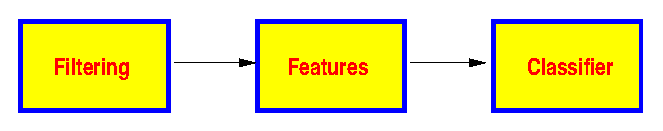
\includegraphics [height=20mm] {bildchen}
\caption {Aufbau eines Mustererkennungssystems}
\end{figure}

\subsection{Erstellen von Tabellen}

Das Volk hat gesprochen:

\begin{table}[h]
\centering
\begin{tabular} {|llc||r|}
	\hline
	Zuname & Vorname & Fraktion & Stimmenanteil \\
	\hline
	Mobutu & General & CDU & 57\% \\
	Tsvangirai & Oberst & CSU & 63\% \\
	\hline
\end{tabular}
\caption {Bundestagswahl in Simbabwe}
\end{table}

%
%	... UND NUN NOCH DAS LITERATURVERZEICHNIS
%
\bibliography{../Literatur/lit}{}
\bibliographystyle{alpha}

\end{document}
